\documentclass[12pt]{extarticle}
\usepackage[utf8]{inputenc}
\usepackage{cite}
\usepackage{graphicx}

\usepackage{hyperref}
\hypersetup{
    colorlinks=true,
    linkcolor=blue,
    filecolor=magenta,      
    urlcolor=blue,
}
\setlength\parindent{0pt}

\title{Modeling Clock Errors in Distributed Systems Represented as Finite State Automata}
\author{Brian Rieder and Celeste Neary
\and \href{https://github.com/brian-rieder/clock-error-modeler}{https://github.com/brian-rieder/clock-error-modeler}}
\date{30 April 2019}

\begin{document}

\maketitle

\section{Abstract}

This investigation examines the impact of the introduction of clock errors in perfectly synchronized distributed systems. In a typical distributed system, it is assumed that processes do not share a common clock, but, due to the closeness of these systems, that the clocks between systems are perfectly synchronized. In this context, this assumption is typically valid but could be violated temporarily. This introduction of such an error can significantly impact the performance of a distributed system to the point of failure.\\

By using Python to model, analyze, and transform timed automata, this investigation analyzes the impact of the introduction of an arbitrary clock error at various states of a distributed system. The algorithm developed in this application inserts a positive or negative clock error in a predefined process in order to simulate the impact of the introduction of a delay into a system comprised of multiple processes. 

\section{Project Description}
The project simulates the behavior of multiple concurrent finite state automata (FSA) when a clock-variation error is introduced. It does so by allowing the user to interactively step through the behavior of FSAs input through a predefined JSON configuration file. Errors are introduced at specified points in time that simulate operation of a system when a process is subjected to clock errors. The project was created using Python.\\

The tool consists of two main applications: \verb|modeler.py| and \verb|visualize_fsa.py|. The first application provides the simulation itself. FSAs are provided to the application using a JSON configuration file. There is also a visualization application to convert the JSON representation of the FSAs to state diagrams. Both applications are shown with their inputs and outputs in Figure \ref{fig:block}. The JSON input and output files are explained in more detail in Section \hyperref[sec:config]{2.1.4}.

\begin{figure}[!htbp]
  \begin{center}
  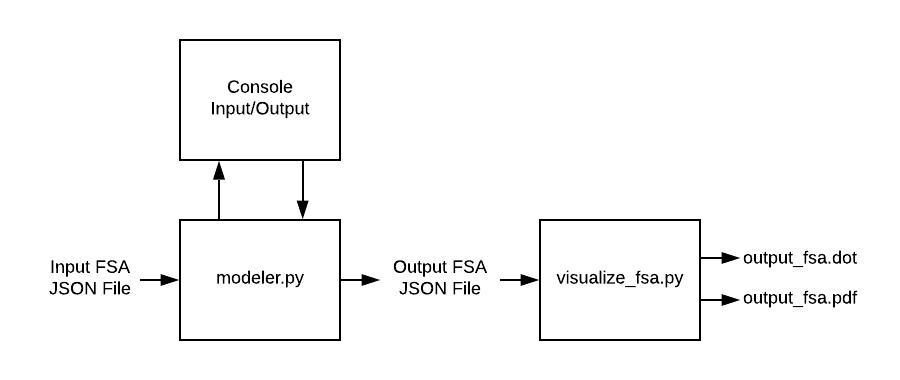
\includegraphics[width=400pt]{./block_diagram.png}
  \end{center}
  \caption{Block diagram for the Clock Error Modeler}
  \label{fig:block}
\end{figure}

The modeler creates a representation of the FSA and allows the user to step through the execution one clock cycle at a time. The console output displays the current state of each process in the system. When the user is done stepping through the FSA, the \verb|quit| command can be used to stop the program and output a modified JSON file.

\subsection{Modeling the Finite State Automata}
The tool can represent one or more processes modeled as finite state automata. This section describes the representation of these automata.
\subsubsection{States and Processes}
States are the building blocks of each process. \verb|State.py| defines the \verb|State| class. Each state includes a name, the name of the process it belongs to, a list of actions, and a list of transitions.

The \verb|State| class also includes methods for constructing each FSA. Essentially, each process is a linked list of \verb|State| objects. The program keeps track of the current state, which contains transitions to potential future states. A complete list of methods is shown in Figure \ref{fig:state}.

\begin{figure}[!htbp]
  \begin{center}
  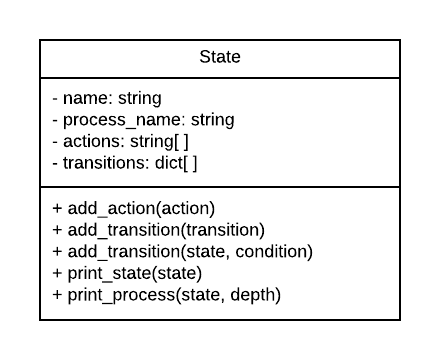
\includegraphics[width=250pt]{./state.png}
  \end{center}
  \vspace*{-10mm}
  \caption{UML State Diagram}
  \label{fig:state}
\end{figure}

Multiple processes are represented using a list of \verb|State| objects, one representing the current state in each process.

\subsubsection{Transitions}
Each process is traversed using state transitions. Each state contains a list of transitions, which are represented by dictionaries. A state with an empty list of transitions is a terminal state.\\

Each dictionary contains a reference to the next state (\verb|State| object), a condition (lambda function), and a condition string.\\

At each clock cycle, the condition is evaluated to determine whether the process will move to the next state. If there are multiple transitions that could occur at the same time, they are prioritized by their order in the list. This is done for every process simultaneously, unless there is a clock error. The behavior during clock errors is described further in Section \hyperref[sec:clkerr]{2.2}.

\subsubsection{Actions}
To further represent the behavior of the FSAs, each state contains actions. These actions are performed on a dictionary of global variables that are shared between the processes. Local variables can also be simulated by adding variables to the dictionary that are only accessed by a single process. Since the actions edit the variables, they are stored as strings instead of lambda functions. When the actions are taken at each clock cycle, the strings are executed using the \verb|exec| function.\\

\subsubsection{Configuration File}\label{sec:config}
The configuration file serves to dictate the structure of the system and its processes as well as to define what the clock errors to be injected are defined as. To do so, the configuration file has three primary sections:
\begin{itemize}
    \item \texttt{config}: Specifies all of the characteristics of where, how long, and in what way the clock errors injected into the system are going to occur.
    \item \texttt{global\_variables}: Section that contains all of the variables accessible to the processes in the system being simulated.
    \item \texttt{processes}: The nodes, edges, and conditions that make up each process.
\end{itemize}

The \texttt{config} section of the configuration file will be detailed further in Section \hyperref[sec:clkerr]{2.2}, but simply indicates which process the clock error will occur in,  how long the error is, when the clock error will occur, and whether or not that process is slower.\\

The \texttt{global\_variables} section of the configuration file simply contains all of the variables that are accessible to the states. These are defined as key-value pairs such that a variable can be referenced by name in conditions and computations. The only requirement for global variables is that they have non-conflicting names and an initial value. It is up to the user to manage their own memory space, so no safeguards or mechanisms for mutual exclusion have been put in place to localize variables or to prevent other processes in the model from altering values used by other processes.\\

The final section, \texttt{processes}, describes the structure of the model and contains three top-level entities:
\begin{itemize}
    \item \texttt{"name"}: Simply the name of the process itself for user reference.
    \item \texttt{"states"}: An array of all states in the system containing their \texttt{"name"} and an array of arithmetic \texttt{"actions"} as defined earlier in this section.
    \item \texttt{"transitions"}: An array of all transitions defining all relations between states, specifying \texttt{"from"} which a state is transitioned \texttt{"to"} under what \texttt{"condition"} as defined earlier in this section.
\end{itemize}
This section is used to create the FSA within the simulation and defines all of the various mechanisms for traversing the system. Of note is that the priority of transitions are the order indicated within the configuration file -  there is no numeric priority, but rather positional priority within the configuration file with the highest priority being at the top of a transition list.

\subsection{Injecting Clock Errors}\label{sec:clkerr}
As the intention of this investigation is to identify failure points in systems, the injection of clock errors into the system is one mechanism for testing the tolerance of a system. Within this utility, the \texttt{config} section of the JSON configuration file dictates where, how long, and in what direction clock variance will occur. This section, defined above is structured with four primary values defined as follows: 
\begin{itemize}
    \item \texttt{"process\_to\_delay"}: The index (starting at 0) of the process that should be affected by the time delay/speed-up.
    \item \texttt{"delay\_amt"}: The amount of delay/speed-up (in units of global time ticks) to be inserted.
    \item \texttt{"time\_of\_delay"}: The time at which to insert the delay/speed-up such that the process is no longer concurrent.
    \item \texttt{"is\_slower"}: Whether or not the process being adjusted is running fast or slow compared to the other processes in the system.
\end{itemize}
The above four configuration items dictate where clock error should be inserted, how much, when, and in what direction, respectively.\\

Clock error manifests itself as a loop upon execution that either allows only a single process to progress (a process running faster than its counterparts) or all processes to progress except for one (a process running slower than its counterparts). The iterative nature of the tool allows these loops to be inserted and immediately obvious to the user, but whose results are also output to a JSON file upon typing \texttt{quit} after execution. An advantage of this is that it allows a user to input multiple clock variance events based on a single unified clock by simply employing concurrent runs. As such, this can be automated in order to robustly test a system, albeit somewhat manual in its present state.

\section{Uppaal}
Uppaal was developed in collaboration between Uppsala University in Sweden and Aalborg University in Denmark as an integrated tool environment for modeling and analysis of networks of timed automata. It has a simple but comprehensive suite of tools for validation and verification of real-time systems and has support for extension of automata with fundamental data types. Uppaal is licensed such that it’s free for non-commercial applications only and requires a paid license for usage in commercial applications.\\

The usage of Uppaal in the context of this investigation was to serve as a modeling platform for both normally time-contingent automata and their error-adjusted adaptations. Uppaal supports verification through time-step simulation and, as such, was used in the context of this assignment to show whether introduction of clock skew errors would cause failures during operation.\\

Although Uppaal was initially considered for modeling the finite state automata, parallel processes in Uppaal cannot be run simultaneously (only one transition can occur at a time). As a consequence of this not being representative of the concurrent nature of distributed systems, usage of the tool was abandoned early on in development despite the power associated with the tool and the verification abilities that come with it. The modeling portion of the tool was recreated (though using JSON in place of XML) and the capability for iterative execution was implemented.

\section{Results}
A basic system consisting of two processes can be found \href{https://github.com/brian-rieder/clock-error-modeler/blob/master/test_fsa.json}{here}. This system, used as an example for execution, can be visualized by \verb|visualize_fsa.py| as shown in Figure \ref{fig:initviz}.\\

\begin{figure}[!htbp]
  \begin{center}
  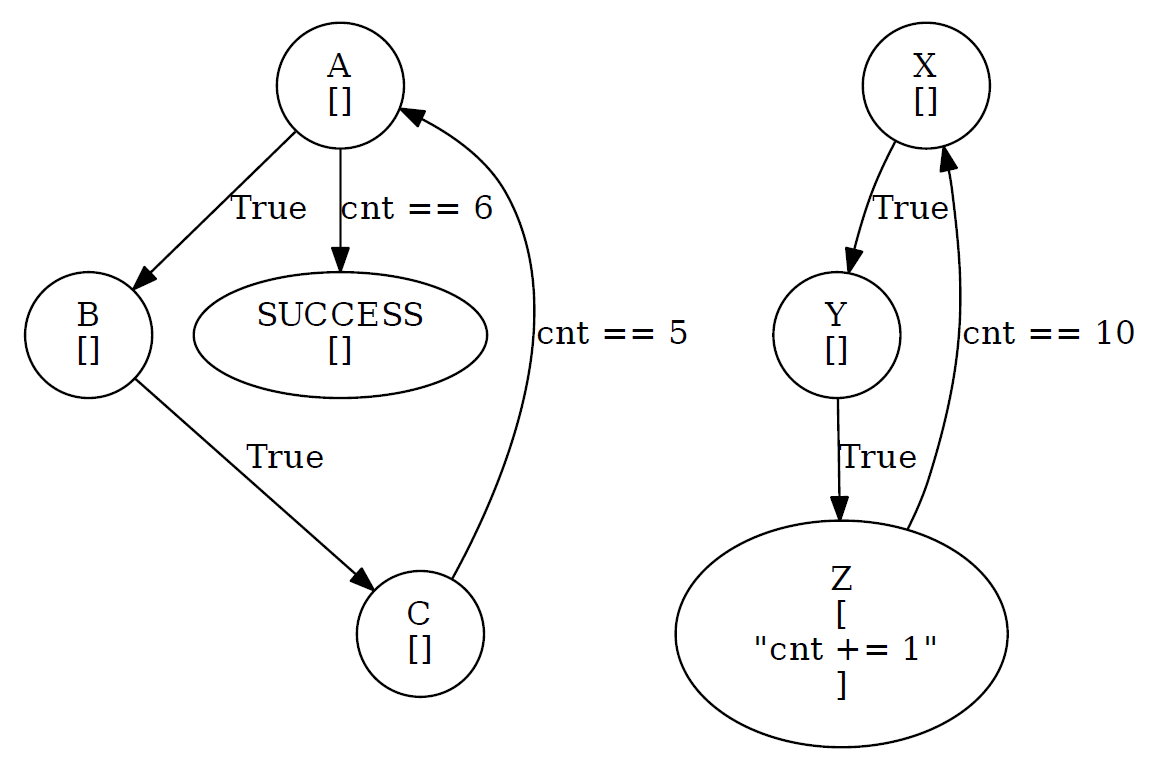
\includegraphics[width=300pt]{./initial.png}
  \end{center}
  \caption{The initial configuration of \texttt{test\_fsa.json}}
  \label{fig:initviz}
\end{figure}

The modeled system, quite simply, iterates to two terminal wait states which both depend on a global variable \texttt{cnt} to be incremented by the second process in state \texttt{Z}. During normal concurrent operation, one would expect that the first process arrives at state \texttt{C} when the second process arrives at state \texttt{X}. The first process waits here until the second process has arrived at \texttt{Z} and begins to increment \texttt{cnt} on every clock tick. Intuitively, one would believe that the transition upon \verb|cnt == 5| would result in the first process transitioning to \texttt{SUCCESS} on the next clock tick. As a result, when run through \texttt{modeler.py} without any delays, the result looks as follows:
\begin{verbatim}
TIME: 14 ------------------------------
{
 "x": 7,
 "cnt": 11
}

State: SUCCESS
State: Z
         State: X , cnt == 10
\end{verbatim}

It is easy to follow, however, that if the first process ever lagged behind such that it missed that transition (or, contrapositively, that the second process was fast enough that it incremented before the first process could ever get there), it could never reach its success state. Showing this failure state is the goal of the tool developed as part of this investigation.\\

In order to model this failure, the following \texttt{config} block was added to the configuration JSON file for the model:
\begin{verbatim}
  "config": {
    "process_to_delay": 0,
    "delay_amt": 5,
    "time_of_delay": 1,
    "is_slower": true
  },
\end{verbatim}
This configuration specifies that the first process should delay for five clock ticks at \verb|time = 1|. This modification can be effectively modeled by the FSA shown in Figure \ref{fig:finalviz}. The consequence of this, as can be shown via \texttt{modeler.py} is a final state which is not \verb|{SUCCESS,Z}|, but rather deadlocked in \verb|{C,Z}|:
\newpage
\begin{verbatim}
TIME: 14 ------------------------------
{
 "cnt": 11,
 "x": 7
}

State: C
         State: A , cnt == 5
State: Z
         State: X , cnt == 10
\end{verbatim}

\begin{figure}[!htbp]
  \begin{center}
  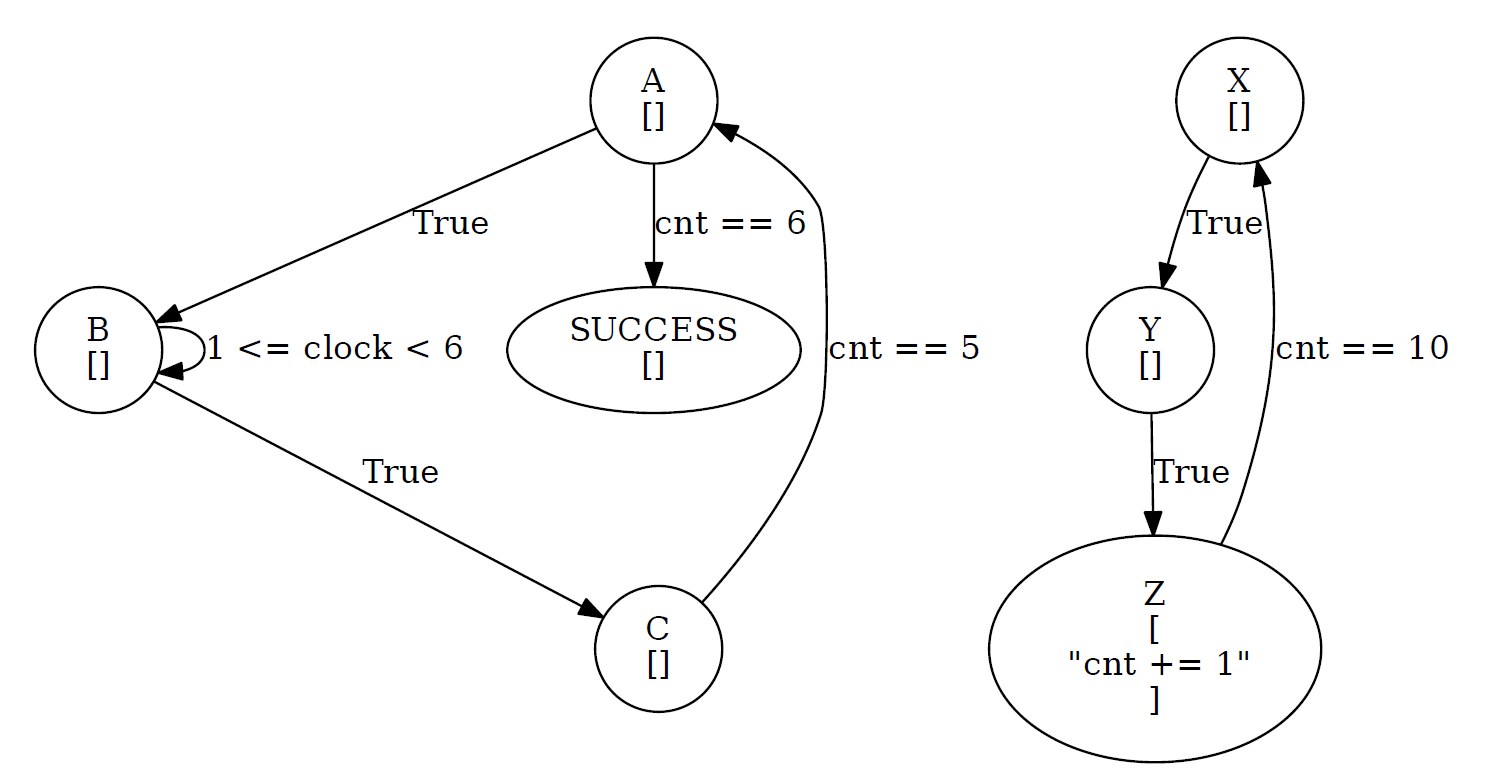
\includegraphics[width=400pt]{./final.png}
  \end{center}
  \caption{The FSA output given a delay of 5 at \texttt{time = 1}.}
  \label{fig:finalviz}
\end{figure}

The intent of the tool is to model and identify these failures as shown above and has been shown to do so effectively given explicit instructions on where failures might occur or where a test case is desired to be imported. As a consequence of the specificity of the location of a potential failure, this utility can be employed programmatically in order to fully test a system, but has potential for future development listed in the next section.

\section{Future Considerations}

The current implementation models one or more state machines that run simultaneously and has the ability to inject a clock error that slows down or speeds up one state machine. Future work can be done to expand upon this project.\\

One consideration is to add more versatility for the clock error injection. The error injection can be randomized to show more in-depth robustness in an algorithm. The randomization can be added to both the time where the delay is inserted and the amount of delay to insert. Introducing variable clock error in a system would allow the user to robustly test a system without being limited to a single configuration per execution.\\

Another consideration is for the model to allow more types of clock errors, such as modeling a system where more than one process is subjected to clock errors or modeling errors that recur over time. While this would significant increase the complexity of the modeling and injection algorithms, the potential in doing so allows for much more representative temporal analysis of the system and identification of failure points in a design.

\end{document}

